% !Mode:: "TeX:UTF-8"
% !TEX program  = xelatex

%\documentclass{cumcmthesis}
\documentclass[withoutpreface,bwprint]{cumcmthesis} %去掉封面与编号页，电子版提交的时候使用。

\usepackage[framemethod=TikZ]{mdframed}
\usepackage{url}   % 网页链接
\usepackage{subcaption} % 子标题
\graphicspath{{figures/}{../dbatzrljy111/outputs/problem1/}}
\title{低轨卫星星座优化部署与鲁棒性设计}
\tihao{A}
\baominghao{202523003030}
\schoolname{电子科技大学}
\membera{唐子然}
\memberb{黄新程}
\memberc{杜彼岸}
\supervisor{本科组}
\yearinput{yy}
\monthinput{mm}
\dayinput{dd}

\begin{document}

\maketitle

\begin{abstract}
背景……问题……\par
\textbf{针对问题一，}……

\textbf{针对问题二，}……

\textbf{针对问题三，}……

\keywords{\textbf{数学建模} \quad  \textbf{图片}\quad   \textbf{表格}\quad  \textbf{公式}}
\end{abstract}

%目录  2019 明确不要目录，我觉得这个规定太好了

%\tableofcontents
%\newpage

\section{问题背景与重述}
\subsection{问题背景}
低轨（LEO）卫星通信星座是指运行在近地低轨道上的通信卫星群，通常由大量卫星分布在多个轨道面上，并通过星间链路共同完成区域或全球通信覆盖。
其具有传输时延低、路径损耗小、终端设备便携、组网灵活等优势，能够更好地支撑多种应用场景，已成为下一代空间信息网络的重要发展方向。
然而，LEO星座的大规模部署会带来星座规模庞大、建设成本高、轨道与频谱资源紧张、星间通信复杂、空间碎片碰撞风险上升等工程挑战。
因此，如何在满足目标区域连续覆盖、低时延通信和故障情况下基本服务能力的前提下，优化星座部署方案、设计合理的星间链路与冗余机制，是低轨卫星星座工程设计中亟需解决的问题。
对该问题进行建模研究，有助于在控制成本的同时提升星座的覆盖性能、通信效率和鲁棒性。
\subsection{问题重述}
现需围绕高度为 $550\,\mathrm{km}$ 左右的低轨通信卫星星座建立数学模型。已知卫星采用近圆轨道，轨道倾角可在 $40^\circ$--$60^\circ$ 内选取；对地通信天线半锥角为 $40.46^\circ$，对应地面覆盖半径约为 $506\,\mathrm{km}$；激光星间链路最大通信距离为 $5000\,\mathrm{km}$；每颗卫星接入容量为 $20\,\mathrm{Gbps}$，星上处理时延为每跳 $0.5\,\mathrm{ms}$。系统设计需满足目标区域内任意地点、任意时刻至少被一颗卫星覆盖，区域内端到端通信时延不超过 $30\,\mathrm{ms}$，并且在任意单颗卫星故障或因碎片规避暂时退出服务时仍保持基本覆盖能力。根据上述条件，本文需要解决以下四个问题。\par

\textbf{问题一：单轨道面覆盖特性分析。}
首先从单颗卫星出发，建立卫星对地覆盖的几何模型，推导覆盖地心角、地面覆盖半径和覆盖面积与轨道高度 $h$、地球半径 $R$、天线半锥角 $\alpha$ 之间的解析关系。其次，将模型扩展到倾角为 $i$、高度为 $h$ 的单个圆轨道面，分析 $N$ 颗均匀分布卫星的星下点轨迹及其随时间变化的规律，并讨论地球自转对目标纬度带连续覆盖的影响。最后，在 $30^\circ\mathrm{N}$--$50^\circ\mathrm{N}$ 纬度带至少存在一颗可见卫星的要求下，确定单轨道面所需的最少卫星数，并刻画卫星间距与覆盖重叠率之间的数量关系。\par

\textbf{问题二：多轨道面星座组网优化设计。}
在单轨道面分析的基础上，考虑由 $M$ 个轨道面组成、各轨道面升交点均匀分布的完整星座。需要先建立星座覆盖性能评估模型，给出覆盖率、平均覆盖重数、最大覆盖间隙时间等指标的定义与计算方法；再以总卫星数量最少为目标，在目标区域 $4^\circ\mathrm{N}$--$53^\circ\mathrm{N}$、$73^\circ\mathrm{E}$--$135^\circ\mathrm{E}$ 内实现全时段单重覆盖，求解轨道面数 $M$、每面卫星数 $N$、轨道倾角 $i$ 以及升交点经度布局；最后进一步考虑 $95\%$ 以上时间内实现二重覆盖的增强要求，比较单重覆盖和二重覆盖方案在星座规模、布局方式和经济成本上的差异。\par

\textbf{问题三：星间链路与通信路由优化。}
在问题二给出的星座方案上，需要构建星间链路网络模型。每颗卫星可连接同轨道面前后相邻卫星，并可连接左右相邻轨道面内距离最近的卫星，且链路距离不超过 $5000\,\mathrm{km}$。因此，需描述轨道运动引起的星间距离周期变化，建立链路通断判据和时变拓扑表示方法。随后，针对目标区域内任意两点之间的通信请求，建立以端到端时延最小为目标的路由策略，综合考虑光速传播时延和星上处理时延，计算平均时延与最大时延并检验是否满足 $30\,\mathrm{ms}$ 约束。进一步地，在单星接入容量受限且业务流量随时间波动的条件下，建立流量分配与拥塞控制模型，评估系统吞吐量和时延表现，并提出流量工程优化建议。\par

\textbf{问题四：碎片规避与星座鲁棒性设计。}
低轨空间碎片会影响星座安全运行，因此需要建立碰撞风险与避撞决策模型。对于单颗卫星，需综合碎片数密度、相对速度、碰撞截面积和预警时间等因素，推导年度平均碰撞概率和预期避撞次数。然后，基于问题二的星座部署方案，估算整个星座一年内的平均避撞次数、避撞机动造成的可用容量下降比例以及相应经济成本。最后，在要求系统 $99\%$ 时间内保持基本覆盖能力的约束下，确定所需冗余卫星数量，并比较每个轨道面增加备用星、增加额外轨道面和设置地面备用卫星三类方案的优劣，给出兼顾覆盖可靠性与成本的冗余配置方案。\par


\section{问题分析}
\subsection{问题一的分析}
问题一要求根据已知参数建立卫星的地面覆盖几何模型，并分析单轨道面卫星对目标纬度带的连续覆盖能力。

对于第一小问，根据卫星、地心与覆盖边界点之间的几何关系，求得覆盖边界对应的地心角，进而计算单颗卫星的地面覆盖半径与覆盖面积。

对于第二小问，首先根据圆轨道运动规律建立卫星星下点的运动模型，描述其纬度和经度随时间的变化。同一轨道面内的卫星均匀分布，可视为以固定相位间隔沿同一轨道运动。结合单星覆盖地心角确定各卫星的纬度覆盖区间，若任意时刻所有区间的并集均能无空隙地覆盖目标纬度带，则认为满足纬度投影意义下的连续覆盖。由于地球自转主要引起星下点经度漂移，而不改变其纬度变化规律，因此不直接影响本问的连续覆盖判定。

对于第三小问，基于第二小问建立的星下点运动模型和连续覆盖判定模型，在一个轨道周期内取样多个时刻，对各卫星的纬度覆盖区间进行计算。在此基础上，对轨道倾角和卫星数进行枚举：先判断该倾角下卫星能否到达目标纬度带上边界，再由少到多搜索满足连续覆盖要求的卫星数，从而得到不同倾角下的最小卫星数。最后，以覆盖区间长度之和与并集长度之差衡量重复覆盖程度，通过改变卫星数，分析相位间隔与覆盖重叠率之间的关系。
\subsection{问题二的分析}
待问题一的单轨道面覆盖模型确定后，问题二将在经纬度二维网格上评价多轨道面星座覆盖性能，并进一步优化轨道面数、每轨卫星数、倾角和升交点经度布局。
\subsection{问题三的分析}
问题三将在问题二星座布局基础上，把卫星看作时变图网络中的节点，利用星间链路距离约束确定边集，并以传播时延和星上处理时延为权重建立最短时延路由模型。
\subsection{问题四的分析}
问题四需要在覆盖模型和星座布局基础上叠加碎片碰撞风险与卫星临时退出服务情形，通过概率风险评估和冗余配置比较分析星座鲁棒性。



\section{模型假设}

    \begin{enumerate} 
		\item ……
		\item ……
		\item ……
		\item ……
		\item ……
	\end{enumerate}

\section{符号说明}
	\begin{table}[H] %[h]表示在此处添加浮动体，默认为tbf，即页面顶部、底部和空白处添加
		\captionsetup{skip=4pt} % 设置标题与表格的间距为4pt
		\centering
		\setlength{\arrayrulewidth}{1pt} % 设置表格线条宽度为1pt
		\begin{tabular}{ccc}
			\hline
			\makebox[0.15\textwidth][c]{符号} & \makebox[0.6\textwidth][c]{说明} & \makebox[0.15\textwidth][c]{单位} \\ 
			\hline
			$R$ & 地球平均半径 & km \\
			$h$ & 卫星轨道高度 & km \\
			$r_s$ & 卫星到地心距离，$r_s=R+h$ & km \\
			$\alpha$ & 对地通信天线半锥角 & rad 或 $^\circ$ \\
			$\theta$ & 单星覆盖边界相对星下点的地心角 & rad 或 $^\circ$ \\
			$r_c$ & 单星地面覆盖大圆弧半径 & km \\
			$A_c$ & 单星球冠覆盖面积 & $\mathrm{km^2}$ \\
			$i$ & 圆轨道倾角 & $^\circ$ \\
			$a$ & 圆轨道半长轴，$a=R+h$ & km \\
			$\Omega$ & 升交点赤经 & rad 或 $^\circ$ \\
			$N$ & 单个轨道面内均匀分布的卫星数 & 颗 \\
			$u_k(t)$ & 第 $k$ 颗卫星在时刻 $t$ 的纬度辐角 & rad \\
			$\varphi_k(t)$ & 第 $k$ 颗卫星的星下点纬度 & rad 或 $^\circ$ \\
			$\lambda_k(t)$ & 第 $k$ 颗卫星的星下点经度 & rad 或 $^\circ$ \\
			$n$ & 圆轨道平均角速度 & rad/s \\
			$T$ & 圆轨道周期 & s 或 min \\
			$\omega_E$ & 地球自转角速度 & rad/s \\
			$C_{\mathrm{lat}}(t)$ & 目标纬度带瞬时纬度投影覆盖率 & 无量纲 \\
			$\Delta u$ & 同轨相邻卫星的相位间隔 & $^\circ$ \\
			$\rho_{\mathrm{red}}$ & 平均冗余覆盖指数 & 无量纲 \\
			$\eta_{\mathrm{ov}}$ & 平均覆盖重叠率 & 无量纲 \\
			$N_{\min}$ & 满足连续覆盖判据的最小单轨卫星数 & 颗 \\
			\hline
		\end{tabular}
	\end{table}

\section{模型的建立与求解}
\subsection{问题一模型的建立与求解}
\subsubsection{单颗卫星地面覆盖模型的建立与求解}
在不考虑地球椭率和地形起伏的条件下，将地球视为半径为 $R$ 的球体，并假设卫星天线波束轴始终指向地心。天线圆锥与地球球面的交线为球面小圆，因此单星覆盖区在地球表面表现为以星下点为球面圆心的球冠；在局部平面投影下，可近似看作圆形区域。

如\cref{fig:q1-single-geometry}所示，记地心、卫星、星下点和覆盖边界点分别为 $O$、$S$、$P$ 和 $B$，则 $OS=R+h$、$OB=R$。天线半锥角为 $\alpha=\angle PSB$，覆盖地心角为 $\theta=\angle POB$。在三角形 $OSB$ 中，$\angle SOB=\theta$，且 $\angle OBS=\pi-\alpha-\theta$。由正弦定理可得
\begin{equation}
    \frac{R}{\sin\alpha}
    =\frac{R+h}{\sin(\alpha+\theta)}.
    \label{eq:q1-sine-law}
\end{equation}
因此，当天线锥边界能够与地球相交，即 $\alpha<\arcsin\!\left(R/(R+h)\right)$ 时，覆盖地心角为
\begin{equation}
    \theta=\arcsin\left(\frac{R+h}{R}\sin\alpha\right)-\alpha .
    \label{eq:q1-theta-alpha}
\end{equation}
覆盖区由球面上与星下点 $P$ 的大圆距离不超过 $R\theta$ 的点组成，故地面覆盖半径与球冠面积分别为
\begin{equation}
    r_c=R\theta,\qquad A_c=2\pi R^2(1-\cos\theta).
    \label{eq:q1-cap-area}
\end{equation}
其中，$r_c$ 为星下点至覆盖边界的球面弧长，$A_c$ 为地球球面上的实际覆盖面积。若忽略地球曲率，覆盖面积可近似为 $\pi r_c^2$；本文在正式计算中采用式\eqref{eq:q1-cap-area}所示的球冠面积。

代入 $R=6371\,\mathrm{km}$、$h=550\,\mathrm{km}$ 和 $\alpha=40.46^\circ$，可得覆盖地心角为 $4.3645^\circ$，地面覆盖半径为 $485.307\,\mathrm{km}$，球冠面积为 $7.39559\times10^5\,\mathrm{km^2}$。题面同时给出地面覆盖半径约为 $506\,\mathrm{km}$；将其作为工程近似参数时，对应地心角为
\begin{equation}
    \theta_g=\frac{506}{R}=4.5506^\circ,
    \label{eq:q1-theta-given}
\end{equation}
相应球冠面积为 $8.03938\times10^5\,\mathrm{km^2}$。两种口径的计算结果见\cref{tab:q1-single-sat}。

\begin{table}[H]
    \caption{单颗卫星覆盖几何参数计算结果}
    \label{tab:q1-single-sat}
    \centering
    \begin{tabular}{lccc}
        \toprule
        计算口径 & 地心角$/({}^\circ)$ & 覆盖半径$/\mathrm{km}$ & 覆盖面积$/\mathrm{km^2}$\\
        \midrule
        几何模型解析值 & 4.3645 & 485.307 & 739558.579\\
        题面工程近似值 & 4.5506 & 506.000 & 803938.086\\
        \bottomrule
    \end{tabular}
\end{table}

\begin{figure}[H]
    \centering
    
\includegraphics[width=0.62\textwidth]{fig_single_satellite_geometry}
    \caption{单颗卫星球面覆盖几何示意（非按比例）}
    \label{fig:q1-single-geometry}
\end{figure}

由\cref{tab:q1-single-sat}可见，几何模型解析半径比题面近似值小约 $4.09\%$。这是因为题目采用“标称 $550\,\mathrm{km}$”和“约 $506\,\mathrm{km}$”的工程化表述，两者并非完全一致。为保持后续计算与题设覆盖能力的参数口径一致，第二、三小问采用题面明确给出的 $506\,\mathrm{km}$ 作为单星覆盖半径；式\eqref{eq:q1-theta-alpha}用于说明覆盖参数与轨道高度、天线半锥角之间的解析关系。

\subsubsection{单轨道面卫星运动与连续覆盖条件}
\noindent\textbf{（1）单颗卫星星下点轨迹模型}

为推导星下点位置，建立地心惯性坐标系 $OXYZ$：原点 $O$ 位于地心，$XY$ 平面为赤道面，$Z$ 轴指向北极，$X$ 轴指向参考方向。记轨道与赤道面的升交点为 $A$，则 $\Omega=\angle XOA$ 为升交点赤经，轨道面绕升交点方向相对赤道面倾斜的角度为轨道倾角 $i$；卫星位置向量与升交点方向之间的夹角记为纬度辐角 $u$。各角度和坐标面的空间关系如\cref{fig:q1-orbit-coordinate}所示。

\begin{figure}[H]
    \centering
    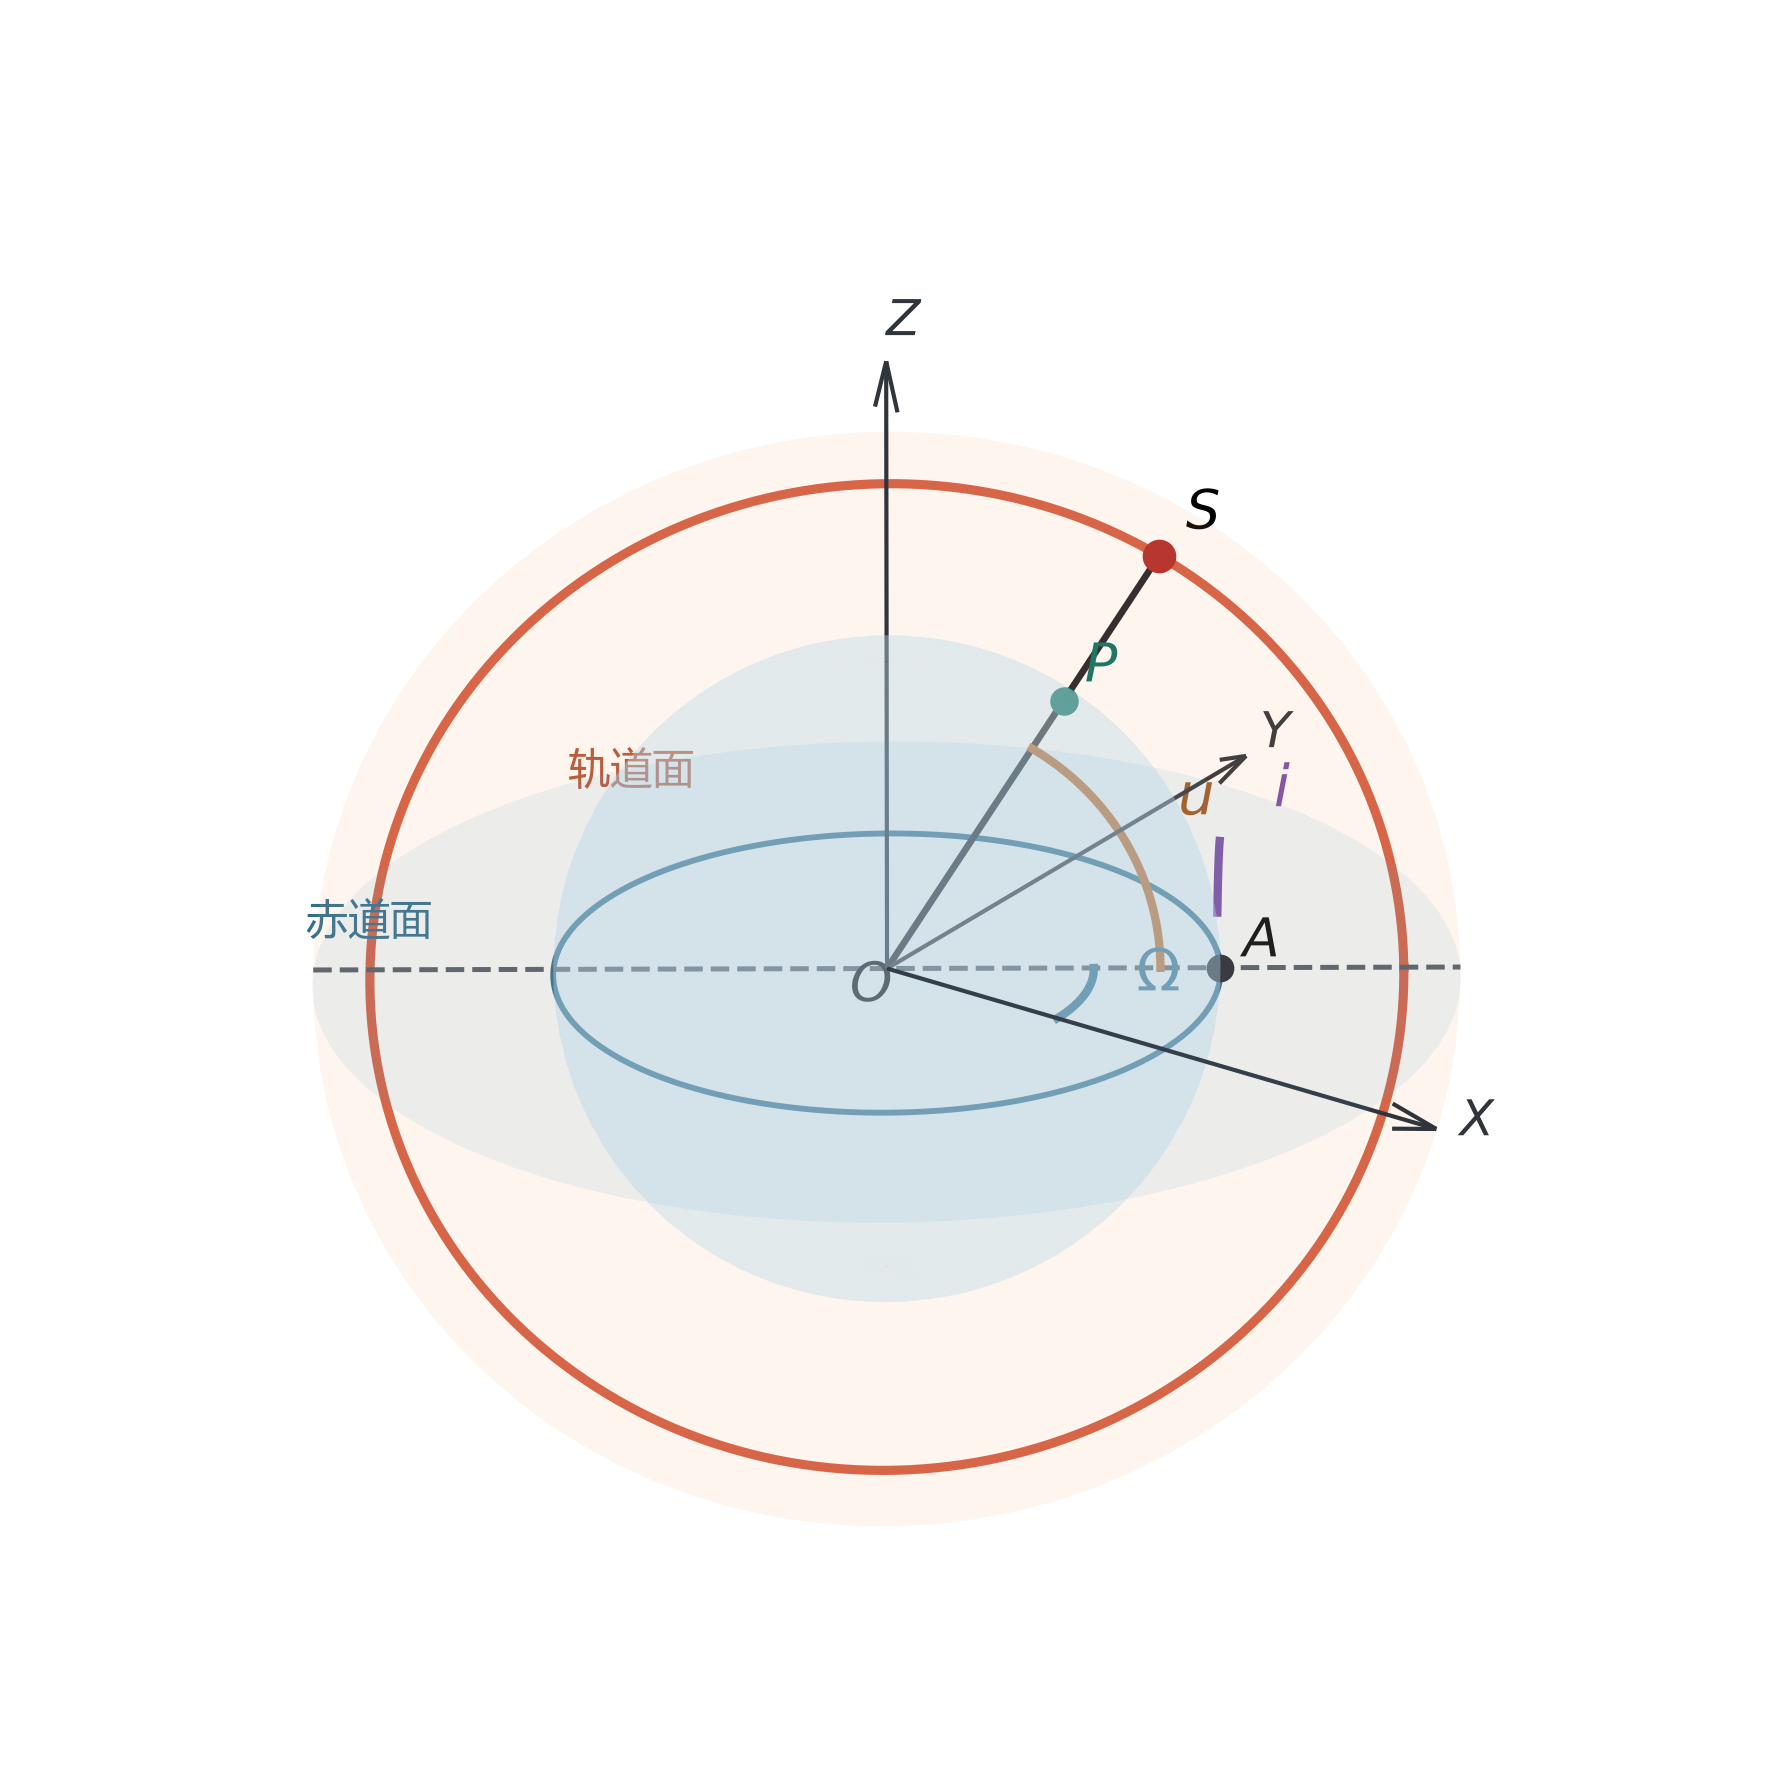
\includegraphics[width=0.72\textwidth]{fig_orbit_coordinate_geometry}
    \caption{圆轨道位置及坐标转换几何关系示意}
    \label{fig:q1-orbit-coordinate}
\end{figure}

将卫星轨道视为高度为 $h$ 的圆轨道，其半长轴为 $a=R+h$。设地球引力常数为 $\mu$，则卫星平均角速度和轨道周期分别为
\begin{equation}
    n=\sqrt{\frac{\mu}{a^3}},\qquad T=\frac{2\pi}{n}.
    \label{eq:q1-orbit-period}
\end{equation}
代入 $R=6371\,\mathrm{km}$、$h=550\,\mathrm{km}$ 和 $\mu=3.986\times10^{14}\,\mathrm{m^3/s^2}$，得到 $T=95.502\,\mathrm{min}$。若初始纬度辐角为 $u_0$，则
\begin{equation}
    u(t)=u_0+nt.
    \label{eq:q1-single-argument}
\end{equation}

在以升交点方向为横轴的轨道平面坐标系中，卫星位置向量可写为
\begin{equation}
    \boldsymbol r_o(t)
    =a\begin{bmatrix}\cos u(t)\\ \sin u(t)\\ 0\end{bmatrix}.
    \label{eq:q1-orbit-position}
\end{equation}
要将其转换到地心惯性坐标系，先绕轨道平面横轴旋转倾角 $i$，再绕 $Z$ 轴旋转升交点赤经 $\Omega$，即
\begin{equation}
    \boldsymbol r_I(t)
    =\boldsymbol R_3(\Omega)\boldsymbol R_1(i)\boldsymbol r_o(t),
    \label{eq:q1-coordinate-rotation}
\end{equation}
其中
\begin{equation}
    \boldsymbol R_1(i)=
    \begin{bmatrix}
        1&0&0\\
        0&\cos i&-\sin i\\
        0&\sin i&\cos i
    \end{bmatrix},\qquad
    \boldsymbol R_3(\Omega)=
    \begin{bmatrix}
        \cos\Omega&-\sin\Omega&0\\
        \sin\Omega&\cos\Omega&0\\
        0&0&1
    \end{bmatrix}.
    \label{eq:q1-rotation-matrices}
\end{equation}
将式\eqref{eq:q1-orbit-position}代入式\eqref{eq:q1-coordinate-rotation}并展开，得到卫星在地心惯性坐标系中的位置
\begin{equation}
    \boldsymbol r_I(t)=a
    \begin{bmatrix}
        \cos\Omega\cos u-\sin\Omega\cos i\sin u\\
        \sin\Omega\cos u+\cos\Omega\cos i\sin u\\
        \sin i\sin u
    \end{bmatrix},
    \label{eq:q1-eci-position}
\end{equation}
其中为简化书写省略了 $u(t)$ 的时间自变量。

在球形地球假设下，星下点 $P$、卫星 $S$ 和地心 $O$ 共线，因此星下点位置向量只是卫星位置向量的径向缩放：
\begin{equation}
    \boldsymbol p_I(t)=\frac{R}{a}\boldsymbol r_I(t).
    \label{eq:q1-subsatellite-vector}
\end{equation}
设 $\boldsymbol p_I=(x_p,y_p,z_p)^{\mathsf T}$，由球面经纬度与直角坐标的转换关系可得
\begin{equation}
    \varphi(t)=\arcsin\!\left(\frac{z_p}{R}\right)
    =\arcsin\!\left(\sin i\sin u(t)\right),
    \label{eq:q1-ground-latitude-single}
\end{equation}
\begin{equation}
    \lambda_I(t)=\operatorname{atan2}(y_p,x_p)
    =\Omega+\operatorname{atan2}\!\left(\cos i\sin u(t),\cos u(t)\right).
    \label{eq:q1-inertial-longitude}
\end{equation}
由上述推导可知，星下点轨迹来自轨道平面位置向量经过倾角和升交点赤经两次旋转后的球面投影。比例因子 $a$ 在计算经纬度时被约去，因此轨道高度不改变星下点的纬度变化范围 $[-i,i]$，但会通过 $n$ 和 $T$ 改变轨迹随时间变化的速度。

\noindent\textbf{（2）同轨多星相位分布模型}

同一轨道面内均匀分布 $N$ 颗卫星时，相邻卫星具有固定相位间隔。第 $k$ 颗卫星的纬度辐角和星下点纬度分别为
\begin{equation}
    u_k(t)=u_0+nt+\frac{2\pi k}{N},\qquad
    \varphi_k(t)=\arcsin\!\left(\sin i\sin u_k(t)\right),
    \quad k=0,1,\ldots,N-1 .
    \label{eq:q1-argument-latitude}
\end{equation}
因此，多颗卫星的星下点轨迹具有相同形状，仅在时间和轨道相位上依次错开。增加卫星数不会改变单颗卫星能够到达的最高纬度，但会减小相位间隔，使各卫星经过目标纬度带的时刻更加密集。

\noindent\textbf{（3）纬度覆盖区间与连续覆盖判据}

第二、三小问采用题面给出的地面覆盖半径 $506\,\mathrm{km}$，即令覆盖地心角 $\theta=4.5506^\circ$。设目标纬度带为
\begin{equation}
    B=[\varphi_a,\varphi_b]=[30^\circ,50^\circ],\qquad
    L_B=\varphi_b-\varphi_a .
    \label{eq:q1-target-band}
\end{equation}
在时刻 $t$，第 $k$ 颗卫星在纬度方向上的覆盖区间为
\begin{equation}
    I_k(t)=\left[\varphi_k(t)-\theta,\ \varphi_k(t)+\theta\right].
    \label{eq:q1-interval}
\end{equation}
目标纬度带在该时刻被连续覆盖的完整条件为
\begin{equation}
    B\subseteq\bigcup_{k=0}^{N-1}I_k(t).
    \label{eq:q1-continuity-condition}
\end{equation}
相邻卫星覆盖区间发生重叠只能说明局部不存在间隙，不能保证目标带上下边界均被覆盖，因此本文采用区间并集进行完整判断。将各区间与 $B$ 求交后，记并集长度为
\begin{equation}
    L_{\mathrm{union}}(t)=
    \left|\bigcup_{k=0}^{N-1}\left(I_k(t)\cap B\right)\right|,
    \label{eq:q1-union-length}
\end{equation}
并定义瞬时纬度投影覆盖率
\begin{equation}
    C_{\mathrm{lat}}(t)=\frac{L_{\mathrm{union}}(t)}{L_B}.
    \label{eq:q1-coverage-rate}
\end{equation}
在一个轨道周期内取 $M$ 个采样时刻 $t_m$。若
\begin{equation}
    \min_{1\leq m\leq M}C_{\mathrm{lat}}(t_m)\geq1-\varepsilon,
    \label{eq:q1-full-coverage}
\end{equation}
则认为该 $(i,N)$ 组合满足纬度投影意义下的连续覆盖要求，其中 $\varepsilon$ 为数值容差。

\noindent\textbf{（4）地球自转影响分析}

地球以角速度 $\omega_E$ 自转时，第 $k$ 颗卫星在地固坐标系中的星下点经度为
\begin{equation}
    \lambda_k(t)=\Omega+
    \operatorname{atan2}\!\left(\cos i\sin u_k(t),\cos u_k(t)\right)-\omega_Et.
    \label{eq:q1-ground-longitude}
\end{equation}
式中，$\operatorname{atan2}$ 用于保证跨象限时经度计算正确。地球自转项只出现在经度表达式中，不改变式\eqref{eq:q1-argument-latitude}给出的星下点纬度，因此不直接影响本问的纬度连续覆盖判据；但它会使相邻轨道周期的地面轨迹产生经度漂移。

\begin{figure}[H]
    \centering
    
\includegraphics[width=0.78\textwidth]{fig_ground_track_example}
    \caption{考虑地球自转的星下点轨迹示例（$i=50^\circ$）}
    \label{fig:q1-ground-track}
\end{figure}

由\cref{fig:q1-ground-track}可见，星下点纬度始终在 $[-i,i]$ 内周期变化，而地面轨迹在经度方向逐圈偏移。因此，本小问建立的纬度判据用于评价单轨道面的基础覆盖能力，完整的二维经纬度区域覆盖将在问题二中进一步分析。

\subsubsection{最小卫星数求解与覆盖重叠分析}
\noindent\textbf{（1）倾角可行性的必要条件}

星下点能够达到的最高纬度为 $i$，考虑单星覆盖地心角后，单轨道面能够触及的最高纬度为 $i+\theta$。要覆盖目标带上边界 $50^\circ\mathrm{N}$，必须满足
\begin{equation}
    i+\theta\geq50^\circ.
    \label{eq:q1-upper-bound}
\end{equation}
该条件仅用于排除几何上不可行的倾角；即使式\eqref{eq:q1-upper-bound}成立，仍需通过一个轨道周期内的区间并集检验判断是否连续覆盖。

\noindent\textbf{（2）最小卫星数枚举求解}

本文在 $40^\circ$--$60^\circ$ 范围内以 $0.25^\circ$ 为步长枚举轨道倾角，在每个倾角下从 $N=1$ 开始递增搜索，并在一个轨道周期内均匀采样 $M=3000$ 个时刻。具体求解过程如下。

Step 1：根据式\eqref{eq:q1-upper-bound}筛除无法达到 $50^\circ\mathrm{N}$ 的倾角。\par
Step 2：对剩余倾角依次枚举 $N=1,2,\ldots,80$，由式\eqref{eq:q1-argument-latitude}计算各卫星在所有采样时刻的星下点纬度。\par
Step 3：构造各卫星的纬度覆盖区间，合并与目标带相交的有效区间，并计算 $C_{\mathrm{lat}}(t_m)$。\par
Step 4：若某一卫星数首次满足式\eqref{eq:q1-full-coverage}，则将其记为该倾角下的最小卫星数 $N_{\min}(i)$。\par

\noindent\textbf{（3）相位间隔与覆盖重叠率计算}

均匀分布卫星的相位间隔为
\begin{equation}
    \Delta u=\frac{360^\circ}{N}.
    \label{eq:q1-spacing}
\end{equation}
在时刻 $t$，各卫星有效覆盖区间长度之和及重复覆盖长度分别定义为
\begin{equation}
    L_{\mathrm{sum}}(t)=\sum_{k=0}^{N-1}\left|I_k(t)\cap B\right|,\qquad
    L_{\mathrm{ov}}(t)=L_{\mathrm{sum}}(t)-L_{\mathrm{union}}(t).
    \label{eq:q1-overlap-length}
\end{equation}
为同时反映重复覆盖的绝对程度与相对程度，定义平均冗余覆盖指数和平均覆盖重叠率为
\begin{equation}
    \rho_{\mathrm{red}}=\frac{1}{M}\sum_{m=1}^{M}
    \frac{L_{\mathrm{ov}}(t_m)}{L_B},\qquad
    \eta_{\mathrm{ov}}=\frac{1}{M}\sum_{m=1}^{M}
    \frac{L_{\mathrm{ov}}(t_m)}{L_{\mathrm{sum}}(t_m)}.
    \label{eq:q1-overlap-ratio}
\end{equation}
其中，当 $L_{\mathrm{sum}}(t_m)=0$ 时，将对应的重叠率项记为 $0$。$\rho_{\mathrm{red}}$ 可以大于 $1$，表示重复覆盖长度相对于目标带宽的倍数；$\eta_{\mathrm{ov}}\in[0,1]$，表示总覆盖长度中重复部分所占比例。固定倾角并改变 $N$，即可得到以 $\Delta u$ 为横坐标、$\eta_{\mathrm{ov}}$ 为纵坐标的关系曲线。

\noindent\textbf{（4）计算结果与分析}

取 $\theta=4.5506^\circ$ 时，由式\eqref{eq:q1-upper-bound}得到倾角至少应达到约 $45.45^\circ$。扫描结果显示，$40^\circ$--$45.25^\circ$ 均因最高覆盖纬度不足而不可行；当倾角刚越过可行边界时，卫星覆盖 $50^\circ\mathrm{N}$ 附近的时间窗口很短，因此仍需较多卫星填补相位空档。

\begin{figure}[H]
    \centering
    
\includegraphics[width=0.80\textwidth]{fig_min_satellites_vs_inclination}
    \caption{不同轨道倾角下满足连续覆盖的最小卫星数}
    \label{fig:q1-min-sat}
\end{figure}

由\cref{fig:q1-min-sat}可见，当倾角增大到 $46^\circ$ 附近时，最小卫星数迅速下降；继续增大倾角后，星下点经过目标带的时间分布发生变化，最小卫星数又逐渐增加。代表性倾角下的搜索结果见\cref{tab:q1-representative}。

\begin{table}[H]
    \caption{代表性倾角下单轨道面连续覆盖结果}
    \label{tab:q1-representative}
    \centering
    \begin{tabular}{cccccc}
        \toprule
        $i/(^\circ)$ & $N_{\min}$ & $\Delta u/(^\circ)$ & $\rho_{\mathrm{red}}$ & $\eta_{\mathrm{ov}}$ & 最长空档/min\\
        \midrule
        45.50 & 76 & 4.737 & 7.7167 & 0.8853 & 0.000\\
        46.00 & 23 & 15.652 & 1.6482 & 0.6224 & 0.000\\
        50.00 & 25 & 14.400 & 1.6606 & 0.6241 & 0.000\\
        55.00 & 30 & 12.000 & 1.4565 & 0.5929 & 0.000\\
        60.00 & 32 & 11.250 & 1.1919 & 0.5437 & 0.000\\
        \bottomrule
    \end{tabular}
\end{table}

由\cref{tab:q1-representative}可知，全部候选倾角中的最小卫星数为 $23$，对应倾角范围为 $46.00^\circ$--$46.75^\circ$。取 $i=46^\circ$、$N=23$ 时，相位间隔为 $15.652^\circ$，一个轨道周期内最长未全覆盖空档为 $0$。

\begin{figure}[H]
    \centering
    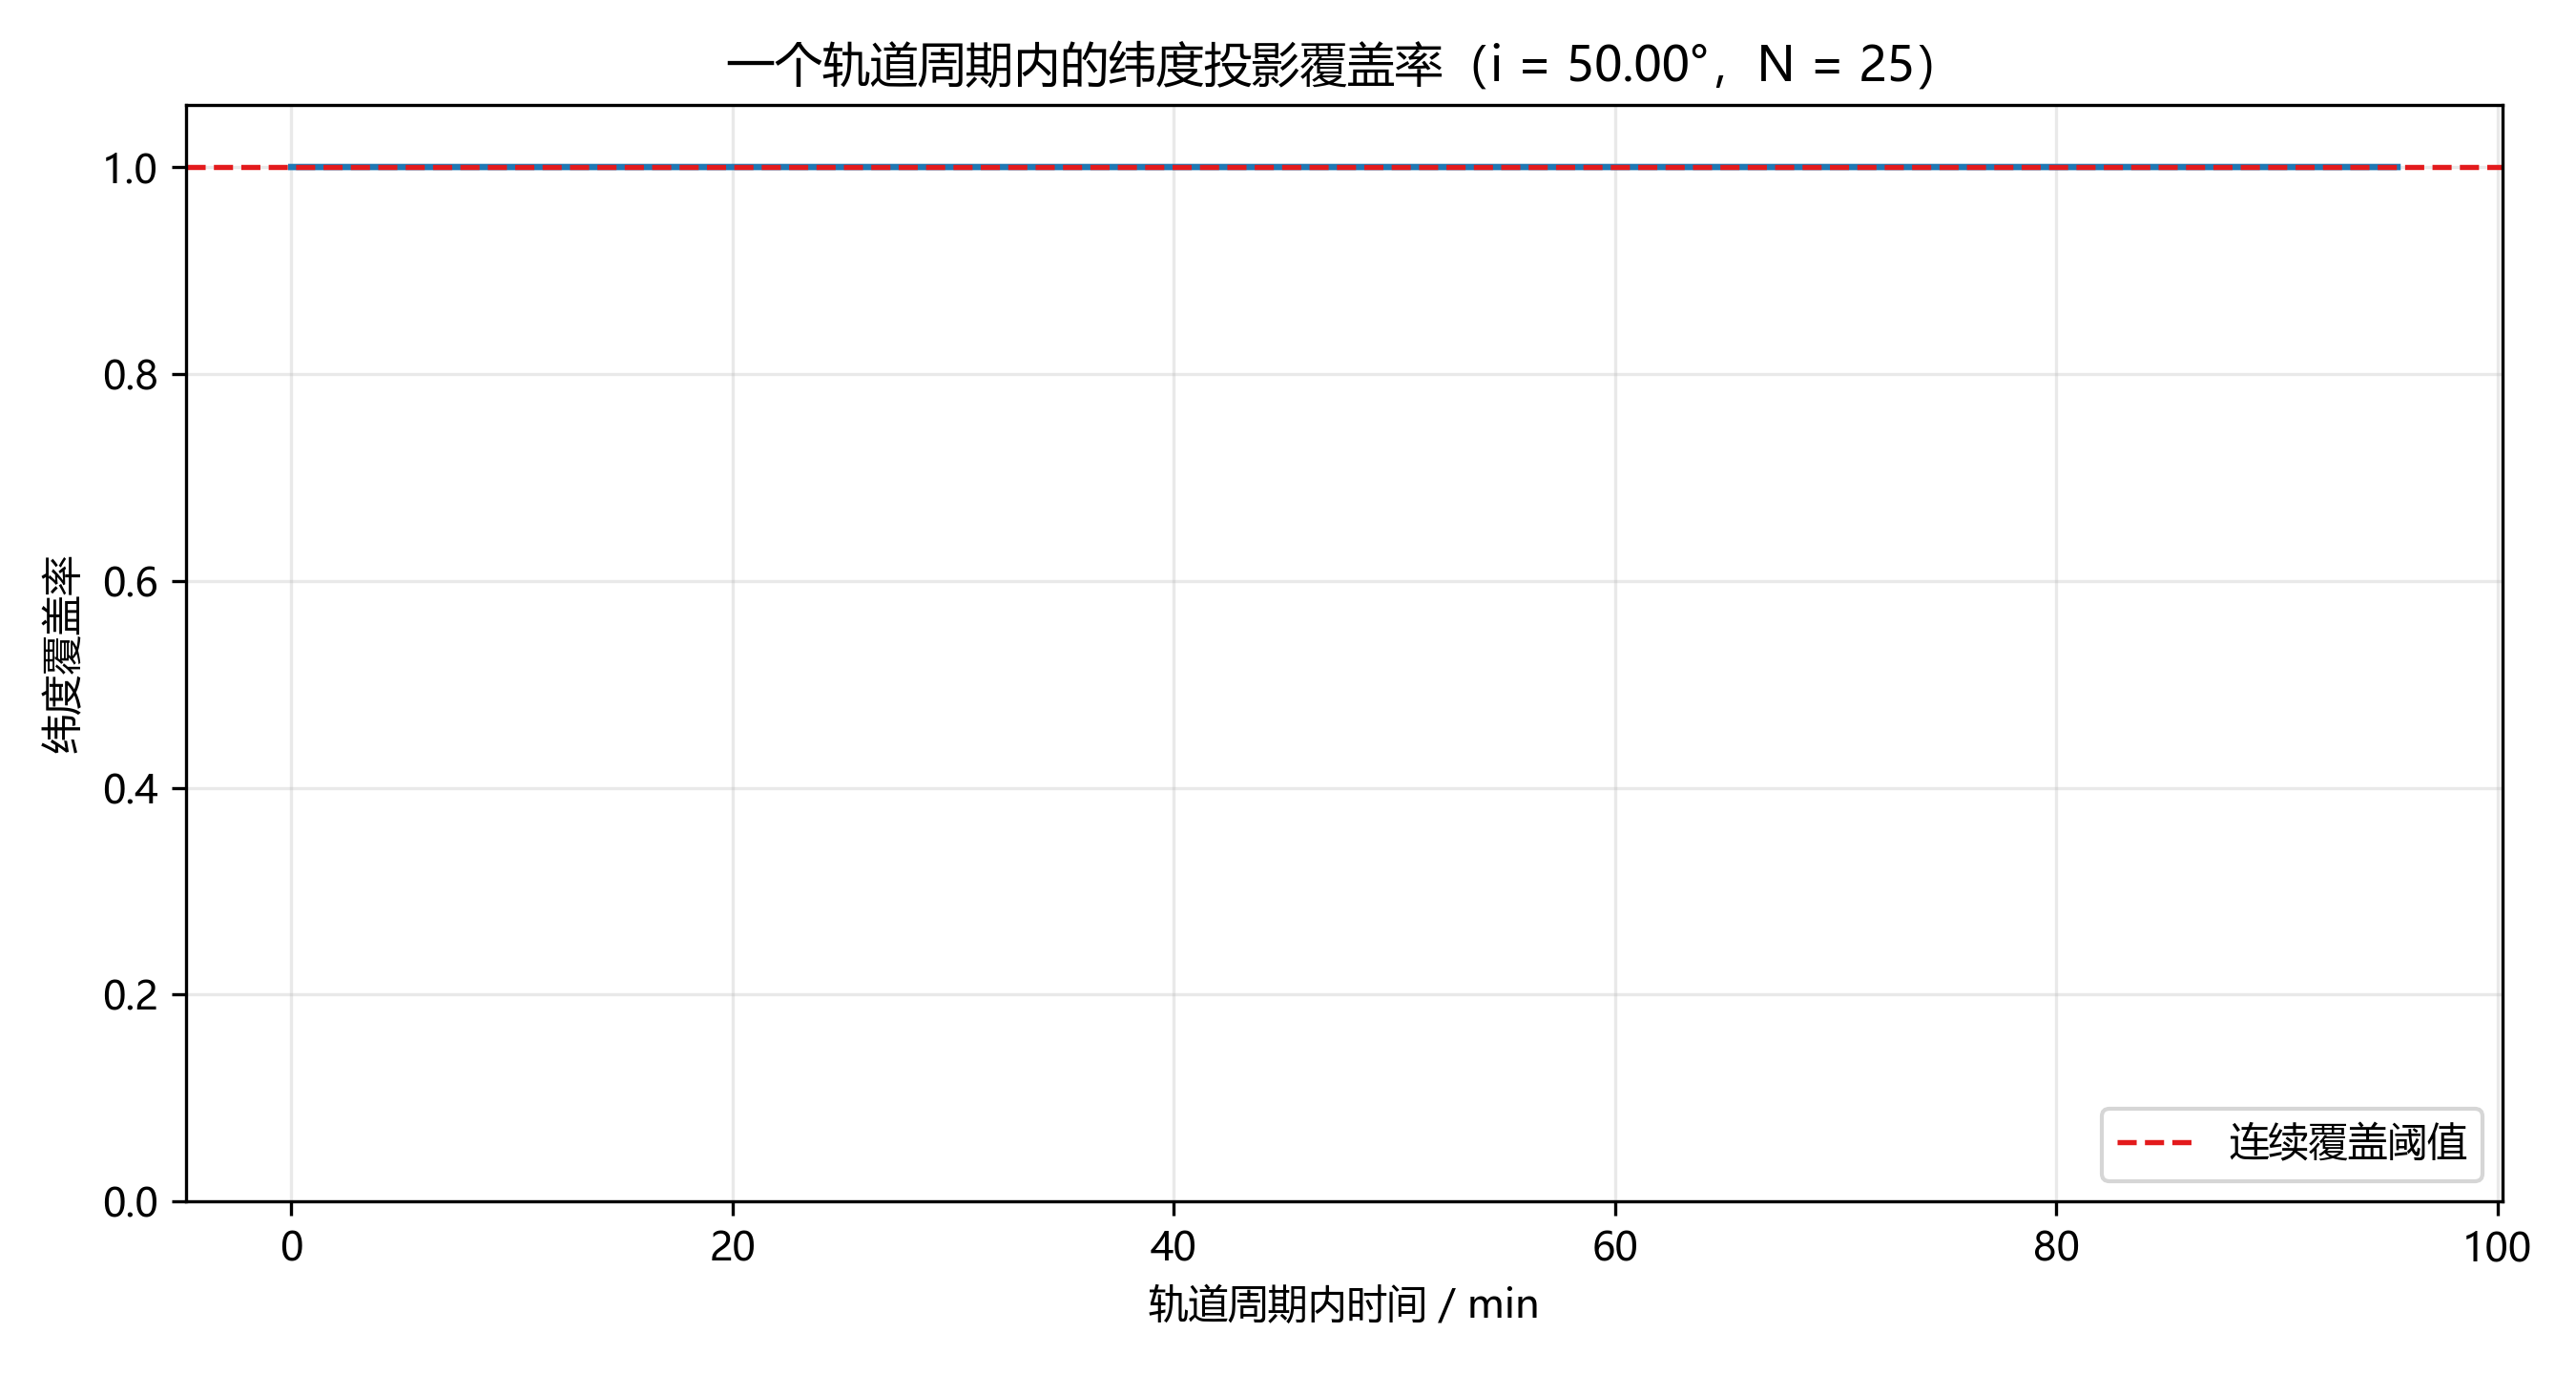
\includegraphics[width=0.80\textwidth]{fig_latitude_coverage_time_example}
    \caption{代表性可行方案在一个轨道周期内的纬度投影覆盖率}
    \label{fig:q1-coverage-time}
\end{figure}

由\cref{fig:q1-coverage-time}可见，代表性方案的 $C_{\mathrm{lat}}(t)$ 在整个轨道周期内始终达到 $1$，说明目标纬度带未出现覆盖空档。

\begin{figure}[H]
    \centering
    
\includegraphics[width=0.80\textwidth]{fig_spacing_redundancy_index}
    \caption{卫星相位间隔与平均覆盖重叠率的关系}
    \label{fig:q1-spacing-overlap}
\end{figure}

由\cref{fig:q1-spacing-overlap}可见，在倾角固定时，随着卫星数增加，相位间隔 $\Delta u$ 减小，平均覆盖重叠率总体上升。这说明缩小相位间隔能够增强覆盖连续性和冗余，但也会提高星座规模与部署成本。综合最小卫星数和连续覆盖结果，问题一推荐采用 $i=46^\circ$、$N=23$ 作为单轨道面基础方案。该结论仅针对 $30^\circ\mathrm{N}$--$50^\circ\mathrm{N}$ 的纬度投影覆盖，完整二维区域覆盖将在问题二中进一步优化。
\subsection{问题二模型的建立与求解}
\subsection{问题三模型的建立与求解}

\section{模型的评价与改进}
\subsection{模型优点}
\subsection{模型缺点}
\subsection{模型改进}
 

%参考文献
\begin{thebibliography}{99}%宽度9
    \bibitem[1]{kaplan1976spacecraft}
    Kaplan M H.
    \newblock Modern Spacecraft Dynamics and Control[M].
    \newblock John Wiley \& Sons, 1976.
    
    \bibitem[2]{luders1961coverage}
    Luders R D.
    \newblock Satellite Networks for Continuous Zonal Coverage[J].
    \newblock The Journal of the Astronautical Sciences, 1961, 7(1): 36-43.
    
    \bibitem[3]{ballard1980rosette}
    Ballard A H.
    \newblock Rosette Constellations of Satellites[J].
    \newblock The Journal of the Astronautical Sciences, 1980, 28(1): 43-54.

    \bibitem[4]{klinkrad2006debris}
    Klinkrad H.
    \newblock Space Debris: Models and Risk Analysis[M].
    \newblock Springer Praxis Publishing, 2006.
\end{thebibliography}

\newpage
%附录
\begin{appendices}

\section{问题一支撑材料说明}
问题一的建模、求解和绘图由 GitHub 项目中的 \path{problem1_latitude_coverage.py} 完成，主要输出位于 \path{outputs/problem1/}。其中，单星覆盖几何参数、不同倾角下的最小卫星数、倾角--卫星数二维扫描结果分别保存为三个 CSV 文件，供正文表格和图形引用。

本文在问题一中引用的主要图片包括：
\begin{enumerate}
    \item \path{fig_single_satellite_geometry.png}：单星球面覆盖几何示意；
    \item \path{fig_orbit_coordinate_geometry.png}：轨道位置与坐标转换几何示意；
    \item \path{fig_ground_track_example.png}：考虑地球自转的星下点轨迹示例；
    \item \path{fig_min_satellites_vs_inclination.png}：不同倾角下的最小单轨卫星数；
    \item \path{fig_latitude_coverage_time_example.png}：代表性可行方案覆盖率随时间变化；
    \item \path{fig_spacing_redundancy_index.png}：相位间距与平均覆盖重叠率关系。
\end{enumerate}
\end{appendices}

\end{document} 
